\documentclass[12pt,a4paper]{report}

\usepackage[utf8]{inputenc}
\usepackage{graphicx}
\usepackage{fancyhdr}
%\usepackage{blindtext}
%\usepackage{showframe}
\usepackage{tikz}
\usetikzlibrary{automata, shapes, positioning, arrows}
\usepackage{tabu}
%%%\usepackage{bookmark}
\usepackage{amsmath}
 %%%%%\bookmarksetup{color=[rgb]{0,0,0}}

\usepackage{lipsum}
\usepackage{tikz-timing}[2014/10/29]
\usetikztiminglibrary{clockarrows}
%%%%%%%%%%%%%%%%%%%%%%%

\definecolor{bgblue}{rgb}{0.41961,0.80784,0.80784}%
\definecolor{bgred}{rgb}{1,0.61569,0.61569}%
\definecolor{fgblue}{rgb}{0,0,0.6}%
\definecolor{fgred}{rgb}{0.6,0,0}%


\usepackage{color}   %May be necessary if you want to color links
\usepackage{hyperref}
\hypersetup{
    colorlinks=true, %set true if you want colored links
    linktoc=all,     %set to all if you want both sections and subsections linked
    linkcolor=black,  %choose some color if you want links to stand out
}






\NewDocumentCommand{\busref}{som}{\texttt{%
#3%
\IfValueTF{#2}{[#2]}{}%
\IfBooleanTF{#1}{\#}{}%
}}

%%%%%%%https://nathantypanski.com/blog/2014-10-29-tikz-timing.html

\newcommand{\comment}[1]{}



 
\renewcommand{\chaptername}{} %% remove the word \chapter

\tikzset{
->, % makes the edges directed
>=stealth, % makes the arrow heads bold
node distance=6cm, % specifies the minimum distance between two nodes. Change if necessary.
%every state/.style={thick, fill=gray!10}, % sets the properties for each ’state’ node
initial text=$reset$, % sets the text that appears on the start arrow
%
}



\tikzstyle{decision} = [diamond, draw, fill=white!20, 
    text width=4.5em, text badly centered, node distance=3cm, inner sep=0pt]
\tikzstyle{block} = [rectangle, draw, fill=white!20, 
    text width=6em, text centered, rounded corners, minimum height=1em]
\tikzstyle{line} = [draw, -latex']
\tikzstyle{cloud} = [draw, ellipse,fill=white!20, node distance=3cm,
    minimum height=4em]
\tikzstyle{arrow} = [thick,->,>=stealth]

\fancyhf{} % sets both header and footer to nothing
\renewcommand{\headrulewidth}{0pt}



\fancypagestyle{logo}{
\fancyhead[RH]{\includegraphics{logo.png}}}
 


\fancyfoot[L]{
\begin{center}
\begin{tabular}{ |c| } 
 \hline
Doc. Name:  Design Document - IIS TRANSMITTER  \hspace{2cm}                    \\
\hline
%Doc. No 1 \hspace{1.5cm}  Doc.Issue No : 01 \hspace{1cm}      Page No : \thepage   \\
\hline
\end{tabular}
\end{center}
}









\begin{document}


\thispagestyle{logo}
\begin{center}

\vspace{20mm}
\textbf{}
\vspace{5mm}
\\
\textbf{}
\vspace{5mm}
\vspace{5mm}
\\ {\large{\textbf{ I2S TRANSMITTER}}} 
\\{\textbf{}}
\vspace{20mm}
%\\
%{\Large{{Hardware Design Group}}}
\vspace{10mm}
%\\
%{\Large{{Centre for Development of Advanced Computing}}}
%\\
\vspace{10mm}
%{\Large{{Thiruvananthapuram}}}
\end{center}
\vspace{105mm}
\hspace{60mm}
\textbf{JUNE 2020}



   \newpage


%\begin{center}
% \begin{tabular}{|c c |} 
% \hline
%Doc. Name & \                                            \  \\ [2ex]
% \hline
% Project  & \                                                \  \\ [2ex]
% \hline
%\end{tabular}
%\end{center}


%\begin{center}
% \begin{tabular}{|c c c c|} 
 %\hline
 %Col1 & Col2 & Col2 & Col3 \\ [0.5ex] 
% \hline\hline
 %1 & 6 & 87837 & 787 \\ 
 %\hline
% 2 & 7 & 78 & 5415 \\
%\hline
% 3 & 545 & 778 & 7507 \\
% \hline
% 4 & 545 & 18744 & 7560 \\
 %\hline
 %5 & 88 & 788 & 6344 \\ [1ex] 
 %\hline
%\end{tabular}
%\end{center}








\tableofcontents
\thispagestyle{logo}
\listoffigures
\thispagestyle{logo}
\listoftables
\thispagestyle{logo}

\pagestyle{logo}
\chapter{Theory, Principle of  Working and Calculations}
\thispagestyle{logo}
\section{I2S protocol}
 Inter-IC sound (I2S)
bus is  a serial link especially for digital audio.The bus handles audio data only, while the other signals, such
as sub-coding and control, are transferred separately. To minimize
the number of pins required and to keep wiring simple, a 3/4-line serial
bus is used consisting of a line for two time-multiplexed data
channels, a word select line and a clock line. In a system I2S master is the device which is generating the clock. The I2S transmitter mentioned here is an I2S master capable of generating the 
clock to an external audio DAC.


\comment {

\begin{figure}[ht]
\begin{tikztimingtable}[%
    timing/dslope=0.2,
    timing/.style={x=5ex,y=2ex},
    x=5ex,
    timing/rowdist=4ex,
    timing/name/.style={font=\sffamily\scriptsize}
]
\busref{SDA}       &    HLlhHlHhlhHl;[dotted]2D{};lllH \\
\busref{SCL}         &  HHLHLHLHLHLHH\\
\extracode
\begin{pgfonlayer}{background}
\begin{scope}[semitransparent ,semithick]
\vertlines[darkgray,dotted]{1,2 ,...,8.0}
\end{scope}
\end{pgfonlayer}
\end{tikztimingtable}
\caption{IIC data transfers}
\end{figure}

}
\section{The I2S bus}
 The bus has three lines:
\begin{itemize}

\item master clock(MCLK)
\item continuous serial clock (SCK)
\item serial data (SD)

\item word select (WS)


\end{itemize}

and the device generating SCK and WS is the master.


\subsection{Master clock (MCLK)}
 The master clock is always an free running clock that is fed to the transmitter to generate the SCK and also to the receiver
as  the oversampling clock. Several I2S receivers are able to generate the MCLK internally thus supporting a 3 wire I2S interface. The I2S master clock is absolutely necessary for jitter free operations. The MCLK is avoided on the ground that it is a fractional clock based on the sampling frequency of the audio data. eg : for 48khz (fs) audio sample the MCLK can be 192fs or 384fs which is 9.216 Mhz or 18.432 Mhz. A clock value of 36.864 Mhz can support most of the sampling frequencies and oversampling requirements.
\subsection{Serial clock (SCK) }
The serial clock is also called the bit clock BCLK in the industry. It is the clock on which the audio data samples are shifted out. The data is shifted on the trailing edge of this clock.
\subsection{Serial Data (SD)}
 The transmitter shifts out the audio data bit by bit on to the SD line on the trailing edge of the SCK. MSB is always transmitted first. The transmitter
always sends the MSB of the next word one clock period after the
WS changes. Such a format is called I2S justified format. Left channel data is shifted during the low period of WS and right channel data is shifted during the high period.
Serial data is always latched on to the
receiver on the leading edge of the serial clock signal, so the transmitter registers the data on SD and WS on the trailing edge of the SCK.
\subsection{Word select (WS)}
The word select signal is also called LRCLK in the industry since this is the signal to identify the left/right audio data on the bus. A low signal indicated left channel is being shifted out and a high signal indicates a right channel audio data on the bus. There is a delay of one SCK period bewteen the serial data and word select signal.


\begin{figure}[ht]
\begin{tikztimingtable}[%
    timing/dslope=0.2,
    timing/.style={x=5ex,y=2ex},
    x=5ex,
    timing/rowdist=4ex,
    timing/name/.style={font=\sffamily\scriptsize}
]
\busref{SCK}         & 14{C} \\
\busref{WS}    & 2H 6L 6H\\
\busref{SD}     & 2U  2D{LSB RIGHT C} 2D{MSB LEFT C} 2U 2D{LSB LEFT C}  2D{MSB RIGHT C} 2U\\ 
\extracode
\begin{pgfonlayer}{background}
\begin{scope}[semitransparent ,semithick]
\vertlines[darkgray,dotted]{1,2 ,...,8.0}
\end{scope}
\end{pgfonlayer}
\end{tikztimingtable}
\caption{3 wire I2S }
\end{figure}


\begin{figure}[ht]
\begin{tikztimingtable}[%
    timing/dslope=0.2,
    timing/.style={x=5ex,y=2ex},
    x=5ex,
    timing/rowdist=4ex,
    timing/name/.style={font=\sffamily\scriptsize}
]
\busref{MCLK}      & 14{C} \\
\busref{SCK}         & 1L 2H 2L 2H  2L 2H  2L 1H    \\
\busref{WS}    & 3H 8L 3H\\
\busref{SD}     & 3U  4D{R} 7D{L}  \\ 
\extracode
\begin{pgfonlayer}{background}
\begin{scope}[semitransparent ,semithick]
\vertlines[darkgray,dotted]{1,2 ,...,8.0}
\end{scope}
\end{pgfonlayer}
\end{tikztimingtable}
\caption{4 wire I2S}
\end{figure}









\section{Advanced Peripheral bus protocol}

The Advanced Peripheral Bus (APB) is part of the Advanced Microcontroller Bus Architecture (AMBA) protocol family. It defines a low-cost interface that is optimized for minimal power consumption and reduced interface complexity. The APB protocol is not pipelined. It is used connect to low-bandwidth peripherals that do not require the high performance of the AXI protocol. The APB protocol relates a signal transition to the rising edge of the clock, to simplify the integration of APB peripherals into any design flow. Every transfer takes at least two cycles.

\subsection{AMBA APB signals}

\begin{itemize}

\item	PCLK     - The rising edge of PCLK times all transfers on the APB.
\item	PRESETn    -The APB reset signal is active LOW. This signal is normally connected directly to the system bus reset signal.
\item	PADDR   -    This is the APB address bus. It can be up to 32 bits wide and is driven by the peripheral bus bridge unit.
\item	PPROT    -   This signal indicates the normal, privileged, or secure protection level of the transaction and whether the transaction is a data access or an instruction access.
\item	PSELx    -   The APB bridge unit generates this signal to each peripheral bus slave. It indicates that the slave device is selected and that a data transfer is required. There is a PSELx signal for each slave.
\item	PENABLE  (APB bridge Enable ) This signal indicates the second and subsequent cycles of an APB transfer.
\item	PWRITE  (APB bridge Direction) - This signal indicates an APB write access when HIGH and an APB read access when LOW.
\item	PWDATA (APB bridge Write data) - This bus is driven by the peripheral bus bridge unit  during     write  cycles when PWRITE is HIGH. This bus can be up to 32 bits wide.
\item	PSTRB  (APB bridge Write strobes)  - This signal indicates which byte lanes to update during a write transfer. There is one write strobe for each eight bits of the write data bus.
\item	PREADY   -  Slave interface Ready. The slave uses this signal to extend an APB transfer.
\item	PRDATA   -  Slave interface Read Data. The selected slave drives this bus during read cycles.
\item	PSLVERR  -  Slave interface error, This signal indicates a transfer failure.


\end{itemize}


\subsection{Write transfers}

There are two types of write transfers:

\begin{itemize}
\item	Write transfer without wait state
\item	Write transfer with wait states
\end{itemize}



A write transfer starts with address PADDR, write data PWDATA, write signal PWRITE, and select signal PSEL, being registered at the rising edge of PCLK. This is called the Setup phase of the write transfer. At the next clock cycle enable signal PENABLE, and ready signal PREADY, are registered at the rising edge of PCLK. 
When asserted, PENABLE indicates the start of the Access phase of the transfer. When asserted, PREADY indicates that the slave can complete the transfer at the next rising edge of PCLK. The address PADDR, write data PWDATA, and control signals all remain valid until the transfer completes. The enable signal PENABLE, is de-asserted at the end of the transfer. The select signal PSEL, is also de-asserted unless the transfer is to be followed immediately by another transfer to the same peripheral

%%%%%%%%%%%%%%%%%%%%%%%%%%%%%%%%%%%%%%%%%%%%%%%%%
%\centering
%\includegraphics[scale=0.8]{AP_WRITE.png}
%\caption{Write transfer with no wait states}

\begin{figure}[ht]
\begin{tikztimingtable}[%
    timing/dslope=0.2,
    timing/.style={x=5ex,y=2ex},
    x=5ex,
    timing/rowdist=4ex,
    timing/name/.style={font=\sffamily\scriptsize}
]
\busref{PCLK}         & 9{C} \\
\busref{PADDR}   & 1L 4D{addr} 4U \\
\busref{PWRITE}      & 1L 4H 4L\\
\busref{PSEL}      & 1L 4H 4L\\
\busref{PENABLE}       & 3L 2H 4L\\
\busref{PWDATA}        & 1L 4D{data} 4U \\
\busref{PREADY}        & 3L 2H 4L\\
\extracode
\begin{pgfonlayer}{background}
\begin{scope}[semitransparent ,semithick]
\vertlines[darkgray,dotted]{1,2 ,...,8.0}
\end{scope}
\end{pgfonlayer}
\end{tikztimingtable}
\caption{Write transfer with no wait states}
\end{figure}

%%%%%%%%%%%%%%%%%%%%%%%%%%%%%%%%%%%%%%%%%%%%%%%%%%%



The PREADY signal can be extended low if the slave device is not able to accept the write transfer, in such a case the PENABLE is extended. Such and transfer is called write transfer with wait states.


\comment {
\begin{figure}[ht]
\centering
\includegraphics[scale=0.8]{AP_WRITE_DELAY.png}
\caption{Write transfer with wait states}
\end{figure}
}

%%%%%%%%%%%%%%%%%%%%%%%%%%%%%%%%%%%%%%%%%%%%%%%%%
%\centering
%\includegraphics[scale=0.8]{AP_WRITE.png}
%\caption{Write transfer with no wait states}

\begin{figure}[ht]
\begin{tikztimingtable}[%
    timing/dslope=0.2,
    timing/.style={x=5ex,y=2ex},
    x=5ex,
    timing/rowdist=4ex,
    timing/name/.style={font=\sffamily\scriptsize}
]
\busref{PCLK}         & 9{C} \\
\busref{PADDR}   & 1L 6D{addr} 2U \\
\busref{PWRITE}      & 1L 6H 2L\\
\busref{PSEL}      & 1L 6H 2L\\
\busref{PENABLE}       & 3L 4H 2L\\
\busref{PWDATA}        & 1L 6D{data} 2U \\
\busref{PREADY}        & 5L 2H 2L\\
\extracode
\begin{pgfonlayer}{background}
\begin{scope}[semitransparent ,semithick]
\vertlines[darkgray,dotted]{1,2 ,...,8.0}
\end{scope}
\end{pgfonlayer}
\end{tikztimingtable}
\caption{Write transfer with wait states}
\end{figure}

%%%%%%%%%%%%%%%%%%%%%%%%%%%%%%%%%%%%%%%%%%%%%%%%%%%




\subsection{Read transfers}

Two types of read transfer are described in this section:
\begin{itemize}
\item With no wait states
\item With wait states.
\end{itemize}
The signals timings for read transfer with and without waits states is shown in the figure.
%%%%%%%%%%%%% \ref{rd_no_wait}.

\comment{
\begin{figure}[ht]
\centering
\includegraphics[scale=1]{READ.png}
\caption{Read transfer with no wait states}
\end{figure}

\begin{figure}[ht]
\centering
\includegraphics[scale=1]{READ_DELAY.png}
\caption{Read transfer with wait states}
%\reference{rd_no_wait}
\end{figure}
}

%%%%%%%%%%%%%%%%%%%%%%%%%%%%%%%%%%%%%%%%%%%%%%%%%%%%%
\begin{figure}[ht]
\begin{tikztimingtable}[%
    timing/dslope=0.2,
    timing/.style={x=5ex,y=2ex},
    x=4ex,
    timing/rowdist=4ex,
    timing/name/.style={font=\sffamily\scriptsize}
]
\busref{PCLK}         & 9{C} \\
\busref{PADDR}   & 1L 4D{addr} 4U \\
\busref{PWRITE}      & 1H 4L 4H\\
\busref{PSEL}      & 1L 4H 4L\\
\busref{PENABLE}       & 3L 2H 4L\\
\busref{PRDATA}        & 1L 4D{data} 4U \\
\busref{PREADY}        & 3L 2H 4L\\
\extracode
\begin{pgfonlayer}{background}
\begin{scope}[semitransparent ,semithick]
\vertlines[darkgray,dotted]{1,2 ,...,8.0}
\end{scope}
\end{pgfonlayer}
\end{tikztimingtable}
\caption{Read transfer with no wait states}
\end{figure}

%%%%%%%%%%%%%%%%%%%%%%%%%%%%%%%%%%%%%%%%%%%%%%%%%%%%%%


\begin{figure}[ht]
\begin{tikztimingtable}[%
    timing/dslope=0.2,
    timing/.style={x=5ex,y=2ex},
    x=4ex,
    timing/rowdist=4ex,
    timing/name/.style={font=\sffamily\scriptsize}
]
\busref{PCLK}         & 9{C} \\
\busref{PADDR}   & 1L 6D{addr} 2U \\
\busref{PWRITE}      & 1H 6L 2H\\
\busref{PSEL}      & 1L 6H 2L\\
\busref{PENABLE}       & 3L 4H 2L\\
\busref{PRDATA}        & 5L 2D{data} 2U \\
\busref{PREADY}        & 5L 2H 2L\\
\extracode
\begin{pgfonlayer}{background}
\begin{scope}[semitransparent ,semithick]
\vertlines[darkgray,dotted]{1,2 ,...,8.0}
\end{scope}
\end{pgfonlayer}
\end{tikztimingtable}
\caption{Read transfer with  wait states}
\end{figure}

%%%%%%%%%%%%%%%%%%%%%%%%%%%%%%%%%%%%%%%%%%%%%%%%%%%%%%%%


\section{Calculations} 


\subsection{Master clock (MCLK)}
The master clock is also called the oversampling clock and is fixed at 36.864 Mhz in the design. So
 \[\textbf{\# }  MCLK = 36.864 Mhz \]

\subsection{Serial/Bit clock (SCK/BCLK)}
The serial/bit clock is generated internally using a divider circuit on the MCLK. The I2S transmitter is limited to the input frequency of the MCLK. For a MCLK of 36.864 Mhz the serial/bit clock possible frequncy is dependent on the sampling frequency of  the audio sample. This clock is designed to be programmed based on the audio specification required. Some of the configurations are :

The exact values of SCK for various audio sampling frequencies is given in the table \ref{tab:SCK}.
\begin{table} 
\begin{center}
\begin{tabular}{|c|c|c|c|c|c|c| } 
 \hline
Audio sample Bit Resolution  &  8Khz &  16Khz  &  48Khz  &  96Khz & 192Khz & 384Khz \\ 
\hline
16 &  0.256   &  0.512  &   1.536  & 3.072 &  6.144   & 12.288 \\
 \hline
24 &  0.384    & 0.768   &  2.304  &  4.608  & 9.216  &  18.432 \\
 \hline
32   & 0.512   &  1.024  &   3.072 &   6.144  &  12.288  & 24.576 \\
 \hline
\end{tabular}
\caption{\label{tab:SCK} SCK values (Mhz) for some common audio bit rate and resolution}
\end{center}
\end{table}

For any other non standard audio bit rate and sampling frequency, The value of SCK is calculated as follows :
\\
 \[\textbf{\# }  SCK frequency = (2*Fs*B )\]
\\
where the multiplier 2 is for stereo , Fs is sampling frequency and B is the audio sample bit resolution.
\\For example for 48Khz 16 Bit audio SCK is 2*48*16 = 1.536 Mhz.
\textbf{The multiplier is always 2 in I2S even for mono audio.}
\subsection{Word select/Left-Right clock (WS/LRCLK)}

The word select or the left-rigth clock is always the \textbf{sampling frequency} of the audio signal. For example for 8Khz audio data, WS/LRCLK is 8Khz. It is an non programmable auto generated signal based on the SCK clock. 







\chapter{System Architecture}
\thispagestyle{logo}
The system architecture is shown below. The deisgn consists of the following submodules.
\begin{figure}[ht]
\centering
\includegraphics[scale=0.8]{ARCH.png}
\caption{Block Diagram}
%\reference{rd_no_wait}
\end{figure}

\begin{itemize}
\item	APB TRANSACTOR - The APB transactor is a state machine capable of handling the APB signals on the interface port.The APB transactor provides exact APB timings for read and write transfers and no wait states are involved in the design. The read data is transferred on the  same clock cycle as the PENABLE signal.The APB PPROT, PSLVERR, PSTRB are not used in the current architecture. All data transfers are 32 bit long. This transactor works at the system clock.
\item AUDIO FIFO - 32-bit wide and 16 entry deep asynchronous fifo bewteen the two clock domains. The audio data is such that first left channel audio is to be written then right channel audio. 
\item  I2S Shift logic - The I2S shift logic read the audio data from the fifo and generates the WS and SD signals. 
\item Registers - The system consistes of a set of registers to control the data transfer on the I2S bus. The detailed description of these registers is provided.
\item Clock counter circuit  - A simple clock divider unit is used to change the frequency of the SCK signal depending on the audio sample frequency. Legal values must be provided into the clock divider circuit.
\item Interrupt Control - Generate an active high interrupt when enabled. The interrupt is activated by writing into the interrupt enable register. This is a programmable interrrupt based on the fifo occupancy. A value can be programmed in the fifo water mark register and a interrupt is generated whenever the fifo occupancy falls below the water mark value. It is cleared by reading the status register or by just disabling the interrupt enable bit.
\end{itemize}


\section{Register Descriptions}

\subsection{ENABLE CORE REGISTER (ECR)  [Read/Write] }
\hspace{1.6cm}
\textbf{Address - 0x00}
\\
\hspace{1.6cm}
Writing any non-zero value will enable the I2S core and the core will start SCK , dequeue audio data from AUDIO fifo and shift it out on the SD line.
All other registers if needed  must be configured before enabling the core for normal operation. Reading returns the core enable status (HIGH - core active).

\subsection{AUDIO FIFO (AF) [Write Only] }
\hspace{1.6cm}
\textbf{Address - 0x04}
\\
\hspace{1.6cm}
Write audio data to this address. Maximum audio sample resolution supported is 32bit. Read as zero.
\\
\textbf{The order of data is left right left with left data written always first. }
\\
\textbf{For mono mode this order is meaningless}
\\
\textbf{Stereo data can be made mono by writting zero on the corresponding channel}
\\
\textbf{Some audio DAC support mono out only. For such cases the DAC will handle the audio data and configure the transmitter as for normal stereo mode}



\subsection{SCK COUNTER REGISTER (SCR)  [Read/Write] }
\hspace{1.6cm}
\textbf{Address - 0x08}
\\
\hspace{1.6cm}
Clock divider circuit configure value. The value written is such that :
\\
 \[\textbf{\# }  SCR = (\dfrac{MCLK\_frequency}{2*SCK\_frequency} )\]
Since MCLK is always 36.864 Mhz
 \[\textbf{\# }  SCR = (\dfrac{36.864 * 10^{6}}{2*SCK\_frequency} )\]

where SCK frequency for some of the standard audio bit rate and resolution is depicted in table \ref{tab:SCK}

The exact values for SCR for various audio bit rate and bit resolution is :
\begin{table} [ht]
\begin{center}
\begin{tabular}{|c|c|c|c|c|c|c| } 
 \hline
Audio sample Bit Resolution  &  8Khz &  16Khz  &  48Khz  &  96Khz & 192Khz & 384Khz \\ 
 \hline         
16   &   72   &    36     &  12   &  6  &    3    &   1.5* \\
 \hline
24  &    48  &    24    &   8    &   4   &   2    &   1  \\
 \hline
32  &   36   &   18     &  6    &  3   &  1.5* &   0.75*  \\
\hline
 \end{tabular}
\caption{\label{tab:SCR} SCR values for some common audio bit rate and resolution}
*not supported
\end{center}
\end{table}

\subsection{AUDIO SAMPLE BIT REGISTER  (ASBR)  [Read/Write] }
\hspace{1.6cm}
\textbf{Address - 0x0C}
\\
Write audio sample resolution into this register.Although any values can be written, standard values are 8, 16, 24, 32.





\subsection{AUDIO FIFO RESET  (AFR)  [Write Only] }
\hspace{1.6cm}
\textbf{Address - 0x10}
\\
Writing any non zero value will reset the audio fifo. New data must be written before enabling the core once the reset has been issued. Read as zero.


\subsection{AUDIO FIFO STATUS REGISTER  (AFSR)  [Read Only] }
\hspace{1.6cm}
\textbf{Address - 0x14}

\begin{center}
\begin{tabular}{|c|c|c|c|c| } 
 \hline
 Reserved   & Aud fifo write count & Audio tx complete &  Aud Fifo in Reset &  Aud Fifo Full \\ 
\hline
31:7 & 6:3  &  2 & 1 & 0\\
 \hline
\end{tabular}
\end{center}


\begin{itemize}
\item Audio Fifo Full   -  Audio fifo full bit. A high value indicates that fifo can no more accept any data. Any new data write during fifo full will result in audio data loss
\item Audio Fifo in Reset  -  This bit indicates that the Audio fifo is in reset state and any write should be avoided during this time. It is asserted during power on and during software resetting the audio fifo. A logic high indicates fifo is in reset state.
\item Audio transfer complete - A logic high indicates all the data written in audio fifo is shifted out on the bus. Can be used to ensure complete data transfer before shutting down the core.
\item Audio fifo write count - Indicates the actual number of data entries in the audio fifo.\textbf{Total fifo depth is 16}.
\item Reserved fields - Writing to these fields have no effect. Read as zero.
\end{itemize}

\subsection{INTERRUPT PENDING REGISTER (IPR) [Read Only] }
\hspace{1.6cm}
\textbf{Address - 0x18}
\\
A value of '1' in this register indicates that the interrupt condition has met and the core has asserted the interrupt and is waiting for the external controller to reset this interrupt. This bit is cleared when AFSR register is read.
This bit is only set when the core is enabled, interrupt is enabled and also the interrupt condition is met. This bit is connected externally to the pin also. This purpose of this register is to use polling mode to detect the interrupt condition in an interrupt-less system. Writing to this register have no effect.

\subsection{INTERRUPT ENABLE REGISTER (IER) [Read/Write] }
\hspace{1.6cm}
\textbf{Address - 0x20}
\\
Writing any non zero value will enable the interrupt. This bit can be cleared by writing zero to this register. \textbf{The external interrupt can be disabled by writing zero to this register or by simply reading the AFSR register.}
Reading will return the value written.


\subsection{INTERRUPT WATER MARK REGISTER (IWMR) [Read/Write] }
\hspace{1.6cm}
\textbf{Address - 0x24}
\\
This register contains a 4 bit value for interrupt condition. The value in this register is compared with audio fifo data count and the interrupt is generated.


\section{Interrupt Operation}

The interrupt mode of operation is very simple. A active high interrupt is generated when the interrupt condition is met. There is only one interrupt condition. A value can be programmed in the IWMR register and interrupt is enabled using IER.
For example , if IWMR is programmed with a value of 10 and the interrupt is enabled, an interrupt (logic high) is generated when ever the audio fifo count goes below or becomes equal to 10. Setting a value of zero can be a test for audio fifo empty condition.
The interrupt can be disabled completely in 2 ways :
\begin{itemize}
\item Writing zero in IER.
\item Reading the AFSR.
\end{itemize}

The interrupt can also be snoozed by writing more data into audio fifo so that the number of data in fifo exceeds the water mark value in IWMR register.










\chapter{Software Environment}
\thispagestyle{logo}

Operating the core is very simple.
\begin{enumerate}
\item Calculate counter value and write in SCR. See SCR register specification on how to calculate the SCR value.
\item Write in ASBR the audio sample bit resolution. for 16 bit audio write 16 in ASBR.
\item Reset the audio fifo by writing any non zero value into  AFR.(not necessary if the device is resetted by power on)
\item Check if the audio fifo reset is complete by reading AFSR fifo in reset bit.
\item Enable the interrupt by writing into IER and IWMR.
\item Write some audio data into audio fifo. (A maximum of 16 write can be done if the fifo is empty).
\item Enable the core.
\item Poll the IPR to see if the interrupt condition is met. If interrupt is supported by the external system, then an logic HIGH will be generated on the irq pin and the external commanding unit can start its interrupt service.
\item Disable/ snooze the interrupt.
\item Write audio data into audio fifo.
\item Disable the core.
\item Reset the audio fifo.


\end{enumerate}

\begin{figure}[ht]
\centering
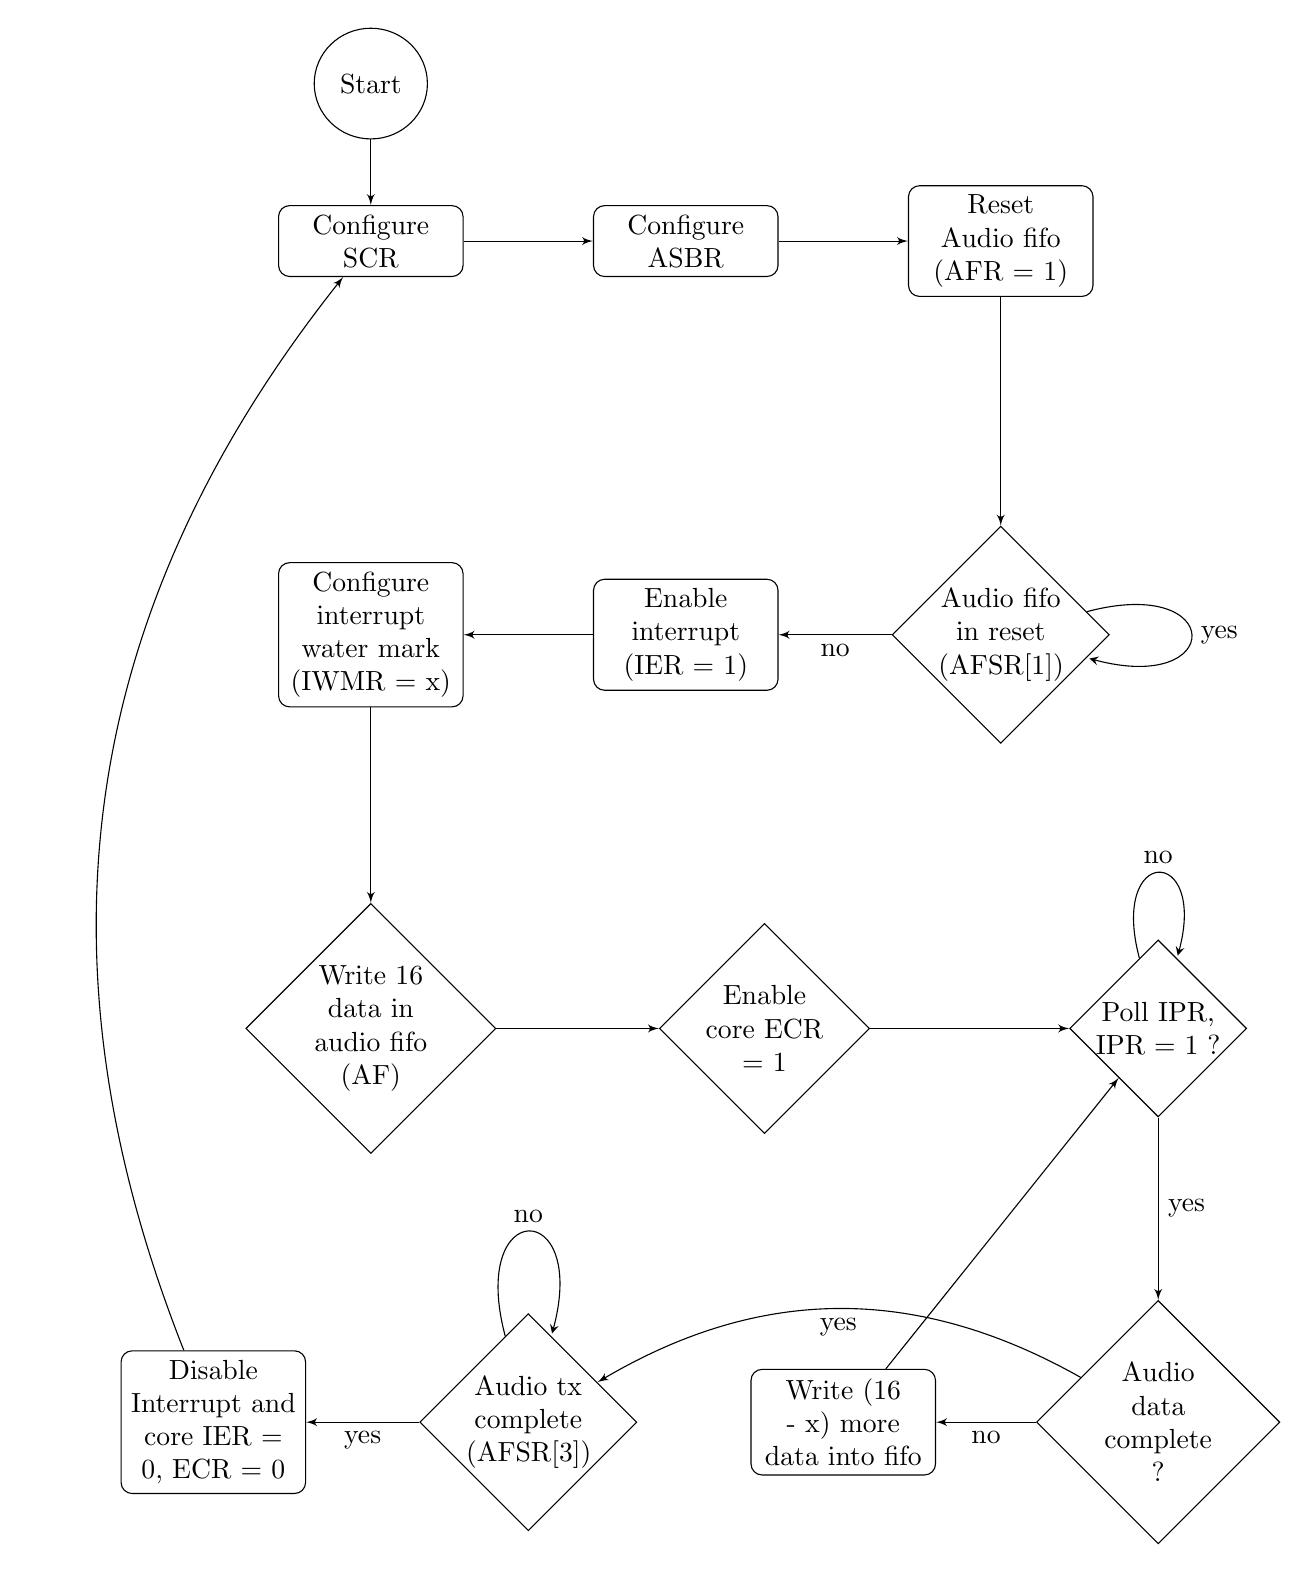
\begin{tikzpicture}[node distance = 2cm, auto]
\node [cloud] (start1) {Start};
\node [block, below of=start1] (scr) {Configure SCR};
\node [block, right of=scr,  node distance=4cm] (asbr) {Configure ASBR};
\node [block, right of=asbr,  node distance=4cm] (reset) {Reset Audio fifo (AFR = 1)};
\node [decision, below of=reset, node distance=5cm] (resetch) {Audio fifo in reset (AFSR[1])};
\node [block, left of=resetch,  node distance=4cm] (ie) {Enable interrupt (IER = 1)};
\node [block, left of=ie,  node distance=4cm] (iwmr) {Configure interrupt  water mark (IWMR = x)};
\node [decision, below of=iwmr, node distance=5cm] (data) {Write 16 data in audio fifo (AF)};
\node [decision, right of=data, node distance=5cm] (enable) {Enable core ECR = 1};
\node [decision, right of=enable, node distance=5cm] (poll) {Poll IPR, IPR = 1 ?};
\node [decision, below of=poll, node distance=5cm] (audc) {Audio data complete ?};
\node [block, left of=audc,  node distance=4cm] (moredata) {Write (16 - x) more data into fifo};
\node [decision, left of=moredata,  node distance=4cm] (txcom) {Audio tx complete (AFSR[3])};
\node [block, left of=txcom,  node distance=4cm] (disable) {Disable Interrupt and core IER = 0, ECR = 0};
%\node [decision, right of=scr, node distance=4cm] (t};

  \path [line] (start1) -- (scr);
  \path [line] (scr) -- (asbr);
  \path [line] (asbr) -- (reset);
  \path [line] (reset) -- (resetch);
  \path [line] (resetch) -- node {no} (ie);
  \draw  [line]  (resetch)  edge[loop right]  node{yes} (resetch);
  \path [line] (ie) -- (iwmr);
  \path [line] (iwmr) -- (data);

  \path [line] (data) -- (enable);
  \path [line] (enable) -- (poll);
  \draw  [line]  (poll)  edge[loop above]  node{no} (poll);
  \path [line] (poll) -- node {yes} (audc);
  \draw  [line]  (audc)  --node{no} (moredata);
 \draw  [line]  (audc)    edge[bend right] node{yes} (txcom);
  \draw  [line]  (disable)  edge[bend left]   (scr);
  \path [line] (moredata) -- (poll);
  \draw  [line]  (txcom)  edge[loop above]  node{no} (txcom);
 \draw  [line]  (txcom)  --node{yes} (disable);

\end{tikzpicture}



\caption{Polling mode of operation}
\end{figure}


\begin{figure}[ht]
\centering
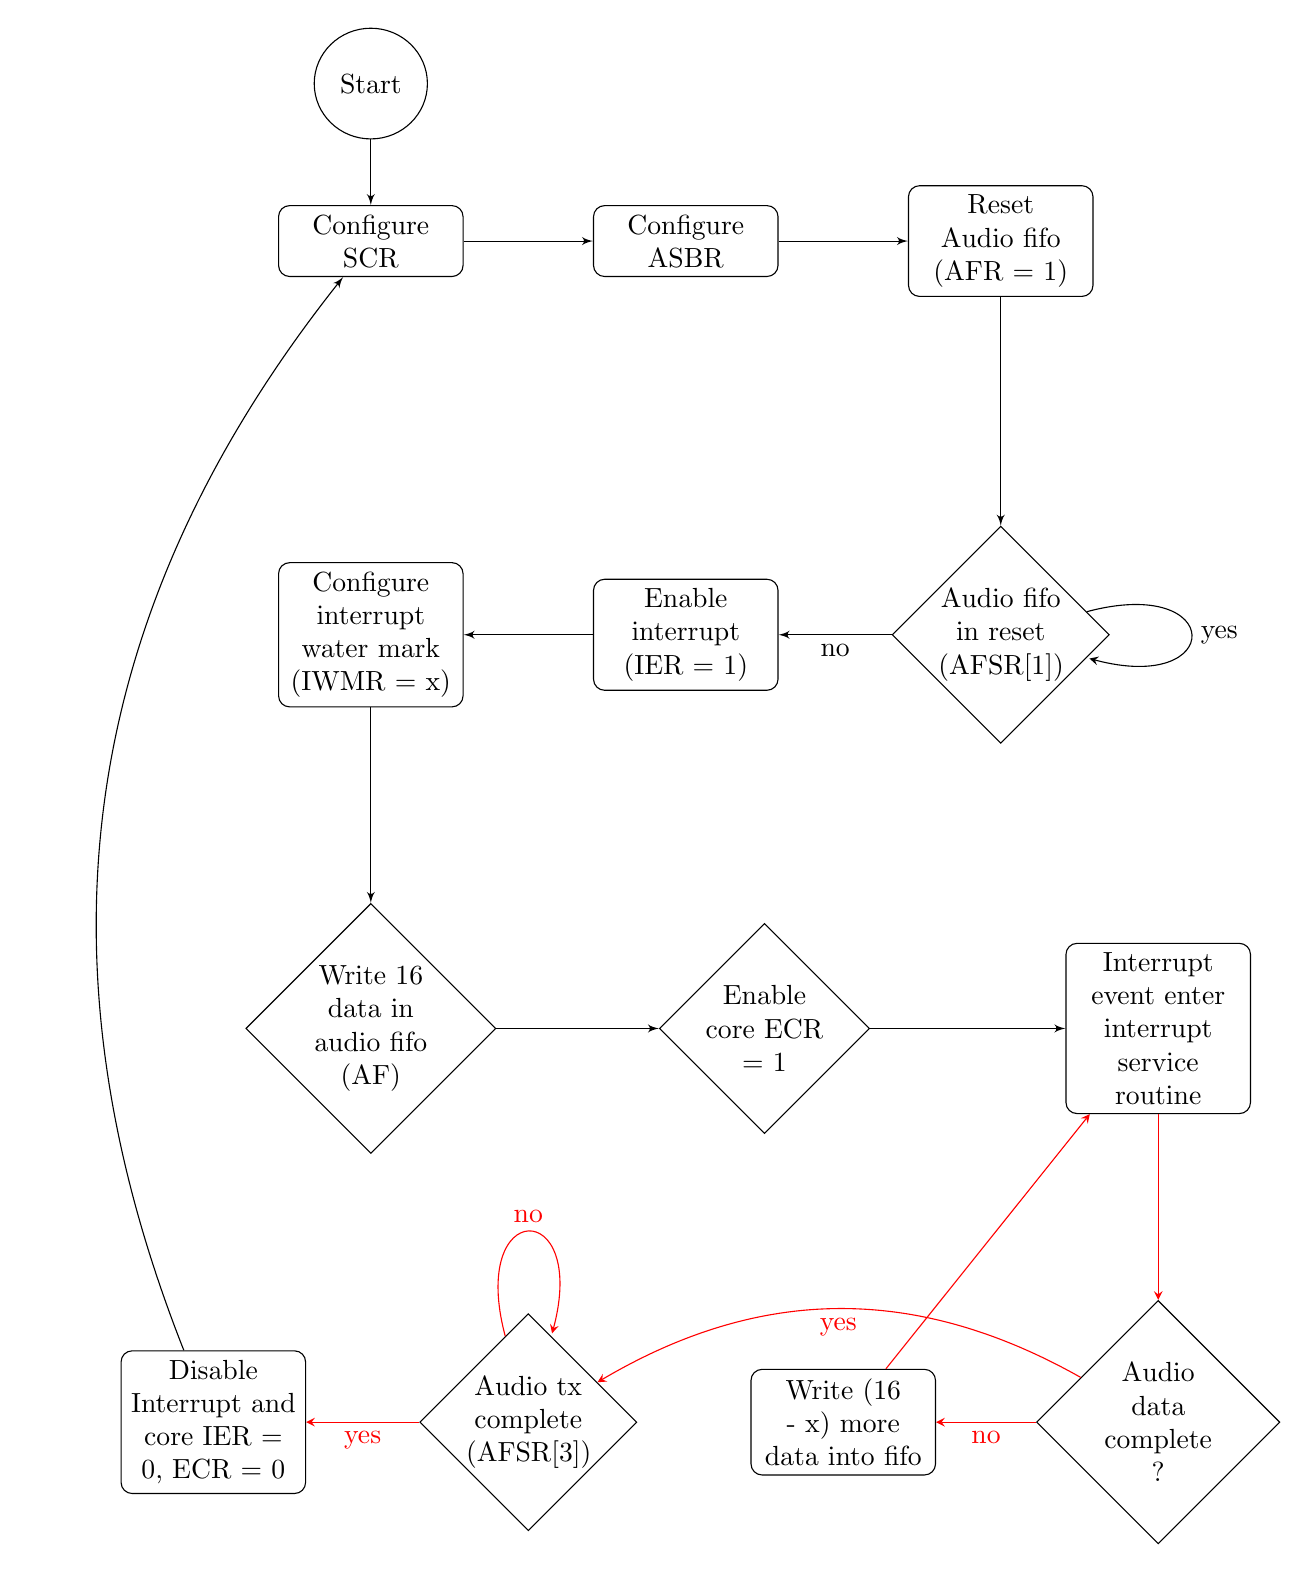
\begin{tikzpicture}[node distance = 2cm, auto]
\node [cloud] (start1) {Start};
\node [block, below of=start1] (scr) {Configure SCR};
\node [block, right of=scr,  node distance=4cm] (asbr) {Configure ASBR};
\node [block, right of=asbr,  node distance=4cm] (reset) {Reset Audio fifo (AFR = 1)};
\node [decision, below of=reset, node distance=5cm] (resetch) {Audio fifo in reset (AFSR[1])};
\node [block, left of=resetch,  node distance=4cm] (ie) {Enable interrupt (IER = 1)};
\node [block, left of=ie,  node distance=4cm] (iwmr) {Configure interrupt  water mark (IWMR = x)};
\node [decision, below of=iwmr, node distance=5cm] (data) {Write 16 data in audio fifo (AF)};
\node [decision, right of=data, node distance=5cm] (enable) {Enable core ECR = 1};
\node [block, right of=enable, node distance=5cm] (poll) {Interrupt event enter interrupt service routine};
\node [decision, below of=poll, node distance=5cm] (audc) {Audio data complete ?};
\node [block, left of=audc,  node distance=4cm] (moredata) {Write (16 - x) more data into fifo};
\node [decision, left of=moredata,  node distance=4cm] (txcom) {Audio tx complete (AFSR[3])};
\node [block, left of=txcom,  node distance=4cm] (disable) {Disable Interrupt and core IER = 0, ECR = 0};
%\node [decision, right of=scr, node distance=4cm] (t};
%\node [decision, right of=scr, node distance=4cm] (t};

  \path [line] (start1) -- (scr);
  \path [line] (scr) -- (asbr);
  \path [line] (asbr) -- (reset);
  \path [line] (reset) -- (resetch);
  \path [line] (resetch) -- node {no} (ie);
  \draw  [line]  (resetch)  edge[loop right]  node{yes} (resetch);
  \path [line] (ie) -- (iwmr);
  \path [line] (iwmr) -- (data);

  \path [line] (data) -- (enable);
  \path [line] (enable) -- (poll);
 
\draw [->,red] (poll) -- (audc);
  \draw [->,red]  (audc)  --node{no} (moredata);
 \draw [->,red] (audc)    edge[bend right] node{yes} (txcom);
  \draw  [line]  (disable)  edge[bend left]   (scr);
 \draw [->,red] (moredata) -- (poll);
  \draw [->,red]  (txcom)  edge[loop above]  node{no} (txcom);
 \draw [->,red] (txcom)  --node{yes} (disable);

%  \draw [->,red] (moredata) -- (poll);

\end{tikzpicture}



\caption{Inerrupt mode of operation : The paths in Red depicts the interrupt service procedure}
\end{figure}

\chapter{Constraining the core}

There are few timing sdc constraints required to time the design. The design has 2 negative edge triggered registers so there are few things to be constrained.
The core is designed in such a way that all the logic is based on leading edge of the sys\_clk and aud\_clk,  however as per protocol requirements the WS and SD signals are shifted to the external pins based on trailing edge of the clock.  Internally WS and SD is generated on the leading edge of the clock and it is just registered on the trailing edge before assigning on the pins. So there will be 2 half cycle paths in the audio domain.
The 2 half cycle paths will not have any combinational circuit.
The timing sdc for the  paths are :

\begin{itemize}
\item set\_half\_cycle\_path    -from */lrclk\_aud\_rp[CK]   -to     */lrclk\_aud\_rn[D]
\item set\_half\_cycle\_path    -from */sdata\_out\_rp[CK]    -to     */sdata\_out\_rn[D]
\item create\_clock -name    audio\_clk -period 27.126 -waveform \{0.0 13.56\}    -source [get\_ports aud\_mclk]
\item  create\_generated\_clock   -name sck   -source    [get\_ports aud\_mclk]   -master\_clock audio\_clk -divide\_by\ 1  [get\_ports sclk\_out ]
\end{itemize}


\end{document}